\setchapterpreamble[u]{\margintoc}
\chapter{Estimating radiometric data from synthetic LiDAR}
\labch{lidar_intensity}
\label{sec:lidar_intensity}

\section*{About this chapter}

This chapter simulates intensity data over the LiDAR simulator explained in the previous chapter. Besides semantic labels, surfaces can also be modelled using multiple BRDFs to estimate additional LiDAR data, such as intensity, multiple returns, etc. At least two approaches are proposed to solve this task. First, it is performed using traditional Computer Graphics BRDFs, whereas a more up-to-date solution operates over the reflectance signature measured from real-world surfaces with a goniophotometer. Another alternative involves transferring LiDAR data into Deep Learning models that help to turn geometrical data into intensity. However, the latter requires solving the LiDAR simulation in the image space by acquiring its depth. Otherwise, point clouds ought to be voxelized, which is not appropriate for collecting LiDAR datasets with a high LOD, or represented with more intricate structures, such as graph-based ones. From the fundamentals of this dissertation, remark that point clouds are unstructured and therefore, Deep Learning is not that flexible when it comes to input data. Nevertheless, this Deep Learning-based alternative is out of the scope of this dissertation, and therefore, we have narrowed this section to the first two proposed approaches.

Comparisons with previous work are not trivial to establish, nor against real-world scans, since the latter requires having the very same model over which the scanning must be performed. Hence, the discussion of this chapter is solely focused on modelling different scenarios with distinct materials. Thus, the evaluation is solely conducted by extracting the density function of every material, to check whether it corresponds to the expected behaviour or not. For instance, TLS scans are able to capture tree trunks with higher density and intensity values, whereas ALS scans are significantly handicapped in this task.  

This chapter solely comprises the description of two approaches on the simulation of LiDAR intensity, based on the previous ToF solver. These are both depicted in the overview of the followed pipeline (Figure \ref{fig:lidar_intensity_overview}).

\section{On the estimation of LiDAR intensity}

The traditional and most straightforward approach for simulating LiDAR radiometry is to use BRDF representations as proposed in Computer Graphics. The number of possible BRDFs is very limited, or at least, these could be not enough to emulate any real-world material. Furthermore, these are constrained to estimating red, green and blue information using the rendering-based material properties, including their albedo and specular factors. Other BRDFs have a larger number of parameters to configure, such as the material roughness and other coefficients. Also, it is not trivial to determine which BRDF is the most similar to emulate one specific material in a synthetic scenario. For instance, Oren-Nayar and Lambertian BRDFs both offer a dull appearance when rendered, thereby hardening the selection of one or another.

\begin{figure}
    \centering
    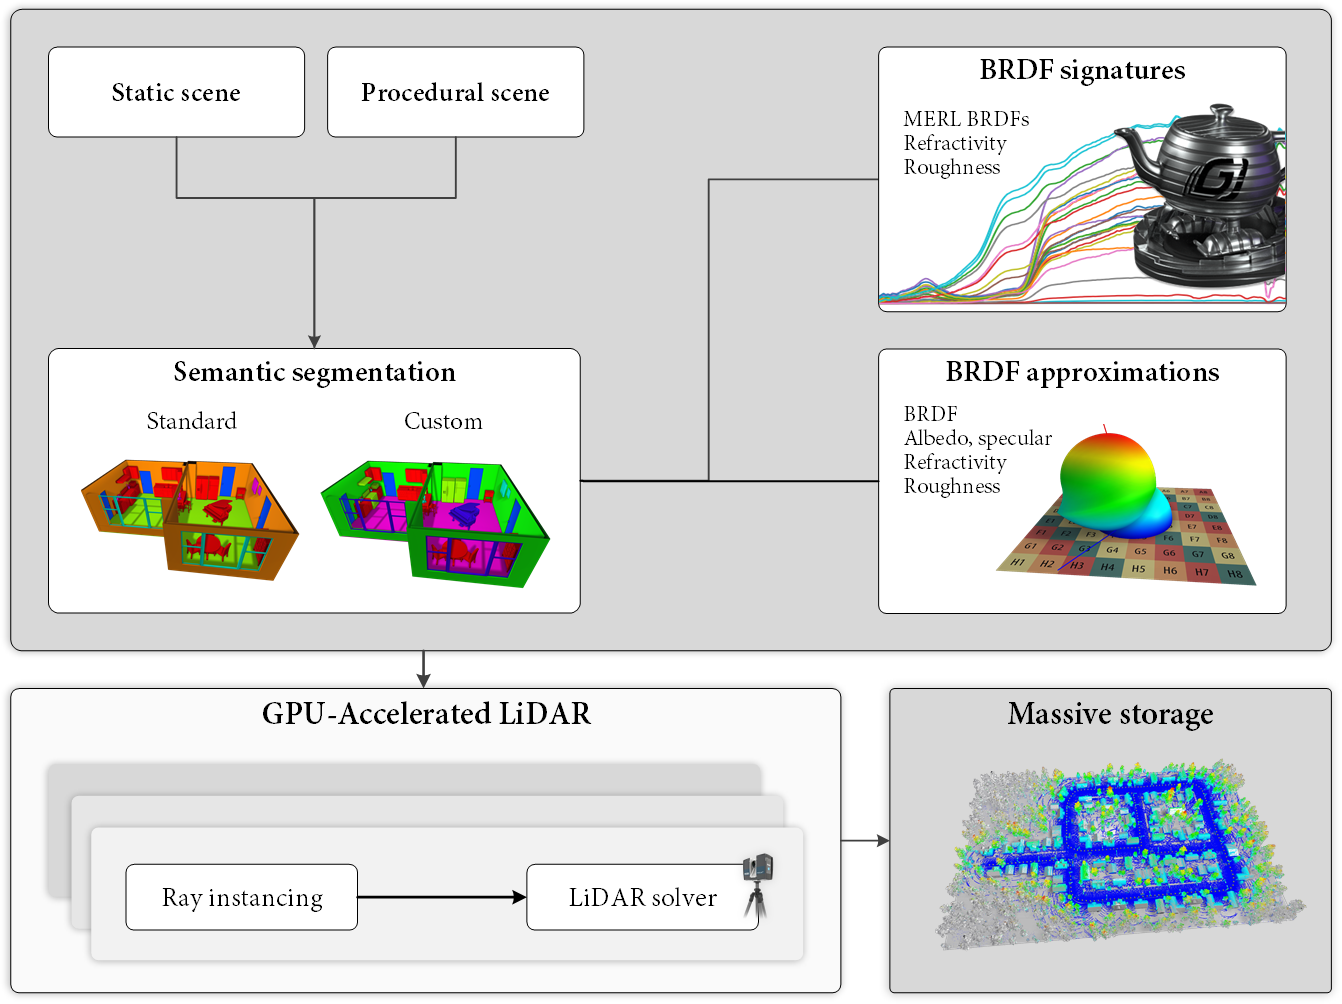
\includegraphics[width=\linewidth]{figs/lidar_intensity/overview.png}
    \caption{Overview of the proposed LiDAR simulation. First, scenes are modelled either as static or procedural, linked to semantic labels as well as to materials properties. Then, a virtual LiDAR iteratively solves the simulation and its result is stored in a standard file format.}
	\label{fig:lidar_intensity_overview}
\end{figure}

More recently, Dupuy and Jakob \cite{dupuy_adaptive_2018} collected a database of spectral signatures concerning isotropic and anisotropic materials. This work captured the spectral interval ranging from 358.628 \si{\nano\meter} to 1001.89 \si{\nano\meter}, with a sampling frequency of $\sim3.341$\si{\nano\meter}, whereas previous work had only provided a database of red, blue, and green wavelengths \cite{matusik_data-driven_2003}. From here, other studies parameterized the collected materials to provide a larger material collection \cite{serrano_intuitive_2016}. However, RGB databases are not appropriate for LiDAR simulations since these sensors operate at wavelengths that suit the target. Accordingly, infrared and near-infrared wavelengths are the most frequent, thereby invalidating the use of RGB collections. Yet, current state-of-the-art hyperspectral databases cannot help to simulate every LiDAR model; for instance, another frequent operating wavelength is 1550 \si{\nano\meter}, which is by far not in the first mentioned interval. These collections are better suited to ray-tracing on the simulation of spectral bands beyond the visible wavelengths, such as the infrared. Nevertheless, this is a more physically-based approach which is expected to provide more similar results to those obtained by LiDAR technology in real-world surfaces.

A brief insight of the literature on the simulation of radiometric data shows the confusion between ray-tracing and ray-casting concepts. To the best of our knowledge, none of previous LiDAR simulators work as a ray-tracing solver; instead, rays are cast and the collision intensity is estimated \cite{ahn_real-time_2020, zhao_method_2021, bechtold_helios_2016}. However, this fusion of ToF and radiometry estimations has led previous work to erroneously refer to this as ray-tracing. Besides this, the operating wavelength has been barely taken into account on the simulation \cite{chen_analysis_2022, gschwandtner_blensor_2011, zohdi_rapid_2020}. Other works use widespread BRDFs such as Oren-Nayar, Lambert and Blinn-Phong \cite{chen_analysis_2022}. More physically-based approaches use material properties such as diffuse, specular and transmissive factors provided by third-party vendors \cite{haider_development_2022}. Finally, another state-of-the-art methods use images co-acquired with LiDAR information to estimate intensity \cite{vacek_learning_2022, xiao_synlidar_2021}. These are typically affected by environmental conditions such as lighting and neither is guaranteed that the material database is large enough. However, the former drawback can be tackled using libraries that help to estimate several environmental and lighting scenarios from a single image \cite{buslaev_albumentations_2020}. Similarly, sensor defects and limitations could be simulated by training a DL model \cite{guillard_learning_2022}.  

\subsection{Model specifications}

\begin{figure*}
    \centering
    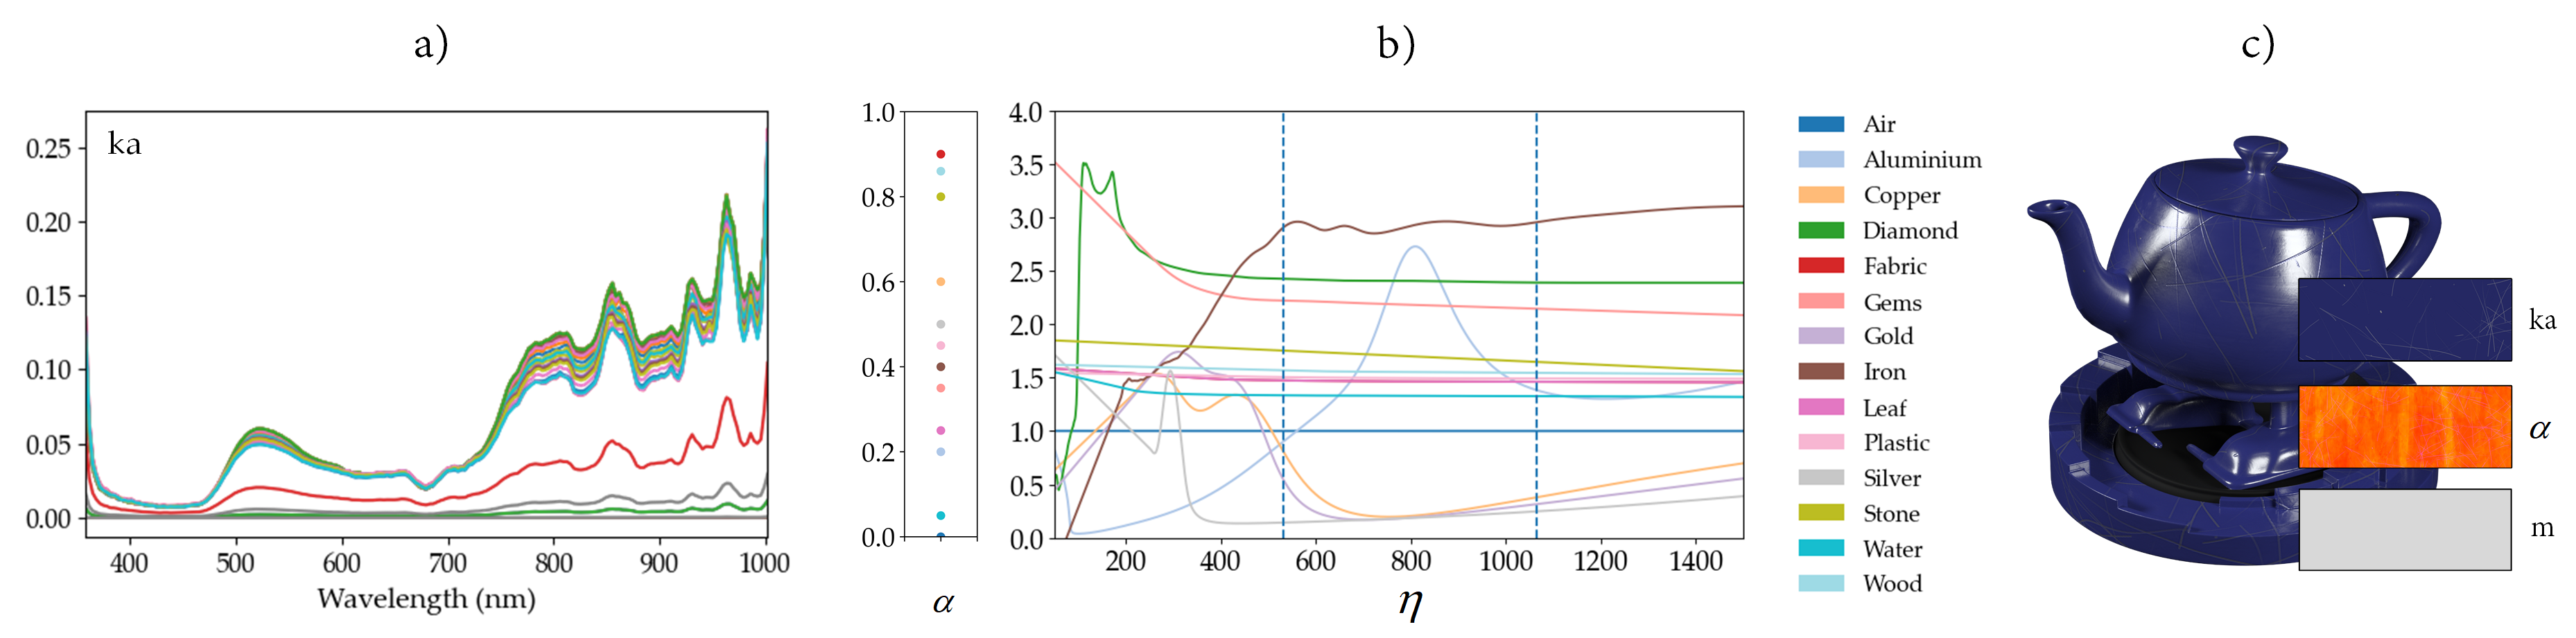
\includegraphics[width=\linewidth]{figs/lidar_intensity/brdf_properties.png}
	\caption{Infrastructure of scene surfaces to calculate LiDAR intensity. a) Reflectance given by BRDFs parameterized with input and output vectors ($w_i$ and $w_o$) \cite{dupuy_adaptive_2018} and b) model-agnostic material specifications, including refractivity and roughness exponent. Finally, c) previously material properties are scaled according to model specifications (albedo, metallic and roughness textures). }
	\label{fig:lidar_brdf_properties}
\end{figure*}

Static and procedural models are linked to semantic annotations and materials aimed at calculating the LiDAR intensity. As previously proposed, materials can also be linked following a hierarchical structure based on model names. This task is facilitated by providing a material database rather than composing every material from scra; instead, a material database is provided representing . Each one of these materials is described with three properties.

Static and procedural models are linked to semantic annotations and materials aimed at calculating the LiDAR intensity. As previously proposed, materials can also be linked following a hierarchical structure based on model names. This task is facilitated by providing a material database rather than composing every material from scratch, since these are defined by three different attributes depicted in Figure \ref{fig:lidar_brdf_properties}. It is composed of some frequent surfaces in the nature (wood, fabric, water, stone, etc.).

Firstly, the ratio between incoming and outcoming radiance for an specific wavelength is provided by a BRDF, thus allowing to better take into account the incidence angle of LiDAR rays. In this task, the emitter, receiver as well as the incident ($\vec{w_{i}}$) and reflected ($\vec{w_{o}}$) vectors are the same, thus reducing the footprint of the BRDF in the GPU. It can be either defined using the goniophotometer measurements or an analytical BRDF. Second, the roughness of a material determines the likelihood of provoking return losses. Finally, the refractive indices can also be obtained from publicly available databases that collect measurements from a large number of sources (most of theem peer-reviewed work) \cite{mikhail_n_polyanskiy_refractive_nodate}. In comparison with the measured BRDFs, refractive indices are provided as sparse values sampled in a variable wavelength range. Hence, these measurements can be used to construct a Catmull-Rom spline which can be later sampled for the specific LiDAR's wavelength. This property is especially relevant for bathymetric LiDAR to account for the refractivity of a new medium.

Note that analytical BRDFs require some properties that are typically provided as PBR textures. However, transferring these textures during the simulation either implies to solve this piece-wise or to build a texture atlas, which present a very limited dimensionality in OpenGL. Instead, the albedo, normal, roughness and metallic factors can be sampled per vertex prior to the simulation, thus storing them in the vertex buffer. This can be efficiently solved with OpenGL's compute shaders.

\begin{figure*}[hbt]
	\centering
	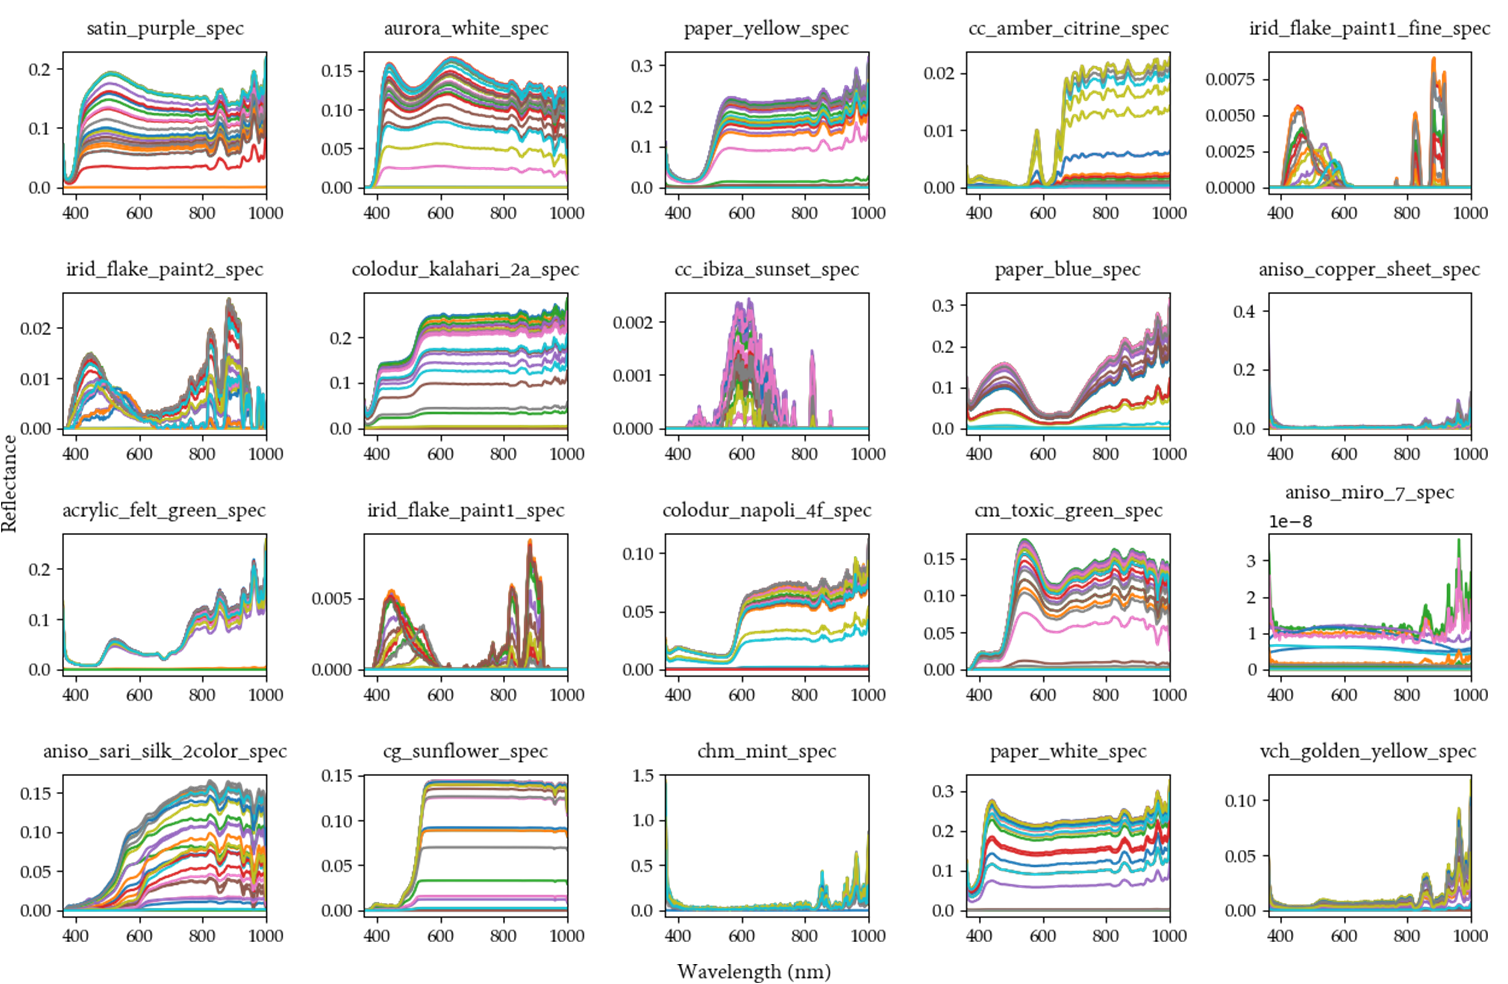
\includegraphics[width=\linewidth]{figs/lidar_intensity/brdf_database_examples.png}
	\caption{Intensity comparison of two procedural environments with different BRDF distributions for an aerial simulation. a) Objects receive the most accurate BRDF in comparison with their real behaviour, whereas b) uses a Lambertian model for every surface. Right images shows the same point cloud rendered according to their relative height and semantic labels, respectively.}
	\label{fig:brdf_merl_examples}
\end{figure*}

\section{Analytical BRDFs}

The surface reflectance is parameterized on the previously presented LiDAR equations. It can be approached with an analytical function, $f_{r}(\vec{w})$, that estimates the amount of light received back to the scanner, according to the incoming energy. Hence, a BRDF can be used for each type of surface, or so to speak, for each material. It computes the ratio between the incoming and outcoming radiance, thus allowing us to better take into account the incidence angle of the laser beams at each point of the virtual environment. In order to cover most of the represented materials, six different BRDFs have been integrated, as depicted in Figure \ref{fig:lidar_analytical_brdfs}.

\begin{marginfigure}[3cm]
    \centering
    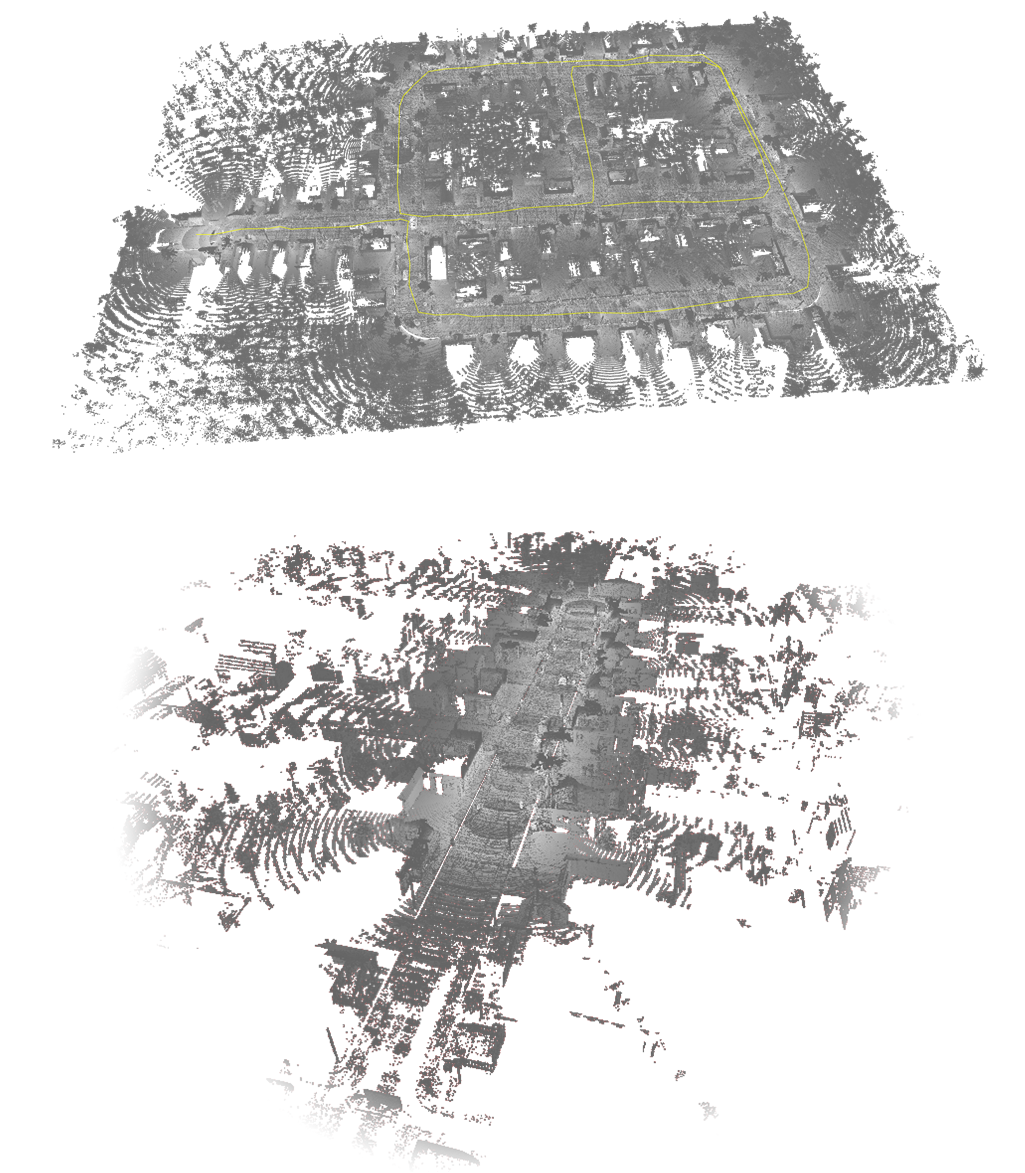
\includegraphics[width=\linewidth]{figs/lidar_intensity/analytical_brdf_intensity_result.png}
    \caption{Some BRDFs depicted. }
	\label{fig:lidar_analytical_brdfs_intensity_result}
\end{marginfigure}
However, these BRDF models tend to simplify when incident and reflected vectors are equivalent, $w_{i} = w_{o}$, as occurs during LiDAR simulations. The following formulae show the backscattering form of the BRDF models depicted in Figure \ref{fig:lidar_analytical_brdfs} and described in \cite{montes_soldado_overview_2012, guarnera_brdf_2016}, where $\rho_{d}$ and $\rho_{s}$ are diffuse and specular colors of the material, and $h$ is the halfway vector ($\hat{l} + \hat{v} = 2w_{o}$, where $\hat{l}$ and $\hat{v}$ are light and view vectors, respectively).

\begin{itemize}
    \item Lambertian: 
    \begin{gather}
        \label{eq:lambert_brdf}
        \begin{aligned}
            f_{r}(\vec{w}) = \frac{\rho_{d}}{\pi}
        \end{aligned}
    \end{gather}
    \item Oren-Nayar: 
    \begin{gather}
        \label{eq:oren_nayar_brdf}
        \begin{aligned}
            f_{r}(\vec{w}) &= \frac{\rho_{d}}{\pi}(A + B)\sin{\theta_{w}} \tan{\theta_{w}}\\
            A &= 1 - 0.5 \frac{{\alpha_{m}^{2}}}{{\alpha_{m}}^2 + 0.33}\\
            B &= 0.45 \frac{{\alpha_{m}^{2}}}{{\alpha_{m}}^2 + 0.09}
        \end{aligned}
    \end{gather}
    \item Minnaert:
    \begin{gather}
        \label{eq:minnaert_brdf}
        \begin{aligned}
            f_{r}(\vec{w}) &= \frac{\rho_{d}}{\pi}(\hat{n} \cdot \hat{w})^{2(k-1)}
        \end{aligned}
    \end{gather}
    \item Blinn-Phong: 
    \begin{gather}
        \label{eq:blinn_phong_brdf}
        \begin{aligned}
            f_{r}(\vec{w}) &= \rho_{s}(\hat{n} \cdot \hat{h})^{k} = \rho_{s}(\hat{n} \cdot 2\hat{w})^{k}
        \end{aligned}
    \end{gather}
    \item Cook-Torrance: 
    \begin{gather}
        \label{eq:cook_torrance_brdf}
        \begin{aligned}
            f_{r}(\vec{w}) &= \frac{F(\beta)D(h)G(\vec{w})}{\pi (\hat{n} \cdot \hat{w})^{2}}\\
            F(\beta) &= F_{0} + (1 - F_{0}) (1 - \hat{n} \cdot \hat{w})^{5}\\
            D(h) &= \frac{1}{\alpha^{2}_{m} (\hat{h} \cdot \hat{n})^{4}} \exp{\frac{(\hat{h} \cdot \hat{n})^{2} - 1}{\alpha^{2}_{m}(\hat{h} \cdot \hat{n})^{4}}}\\
            G(w) &= \min\left(1, \frac{4(\hat{n} \cdot \hat{w})^{2}}{\hat{h} \cdot \hat{w} }\right)
        \end{aligned}
    \end{gather}
    where $F(\beta)$ is the Schlick approximation described by Akenine-Möller et al. \cite{akenine-moller_real-time_2018}, $D(h)$ is the Beckmann distribution \cite{montes_soldado_overview_2012} and $G(h)$ is the geometric attenuation factor. Also note that $F_{0}$ is the external reflection under normal incidence casuistic ($\vec{w} = \vec{n}$), whereas the rest of values are approximated through an interpolation between $F_{0}$ and 1.
    \item Ward anisotropic: 
    \begin{gather}
        \label{eq:ward_brdf}
        \begin{aligned}
            f_{r}(\vec{w}) &= \frac{\rho_{s}\exp\left(-\frac{\left(\frac{h \cdot x}{\alpha_{x}}\right)^{2} + \left(\frac{h \cdot y}{\alpha_{y}}\right)^{2}}{(\hat{h} \cdot \hat{n})^{2}} \right)}{4\pi\alpha_{x}\alpha_{y} (\hat{n} \cdot \hat{w})}
        \end{aligned}
    \end{gather}
\end{itemize}

\begin{figure}
    \centering
    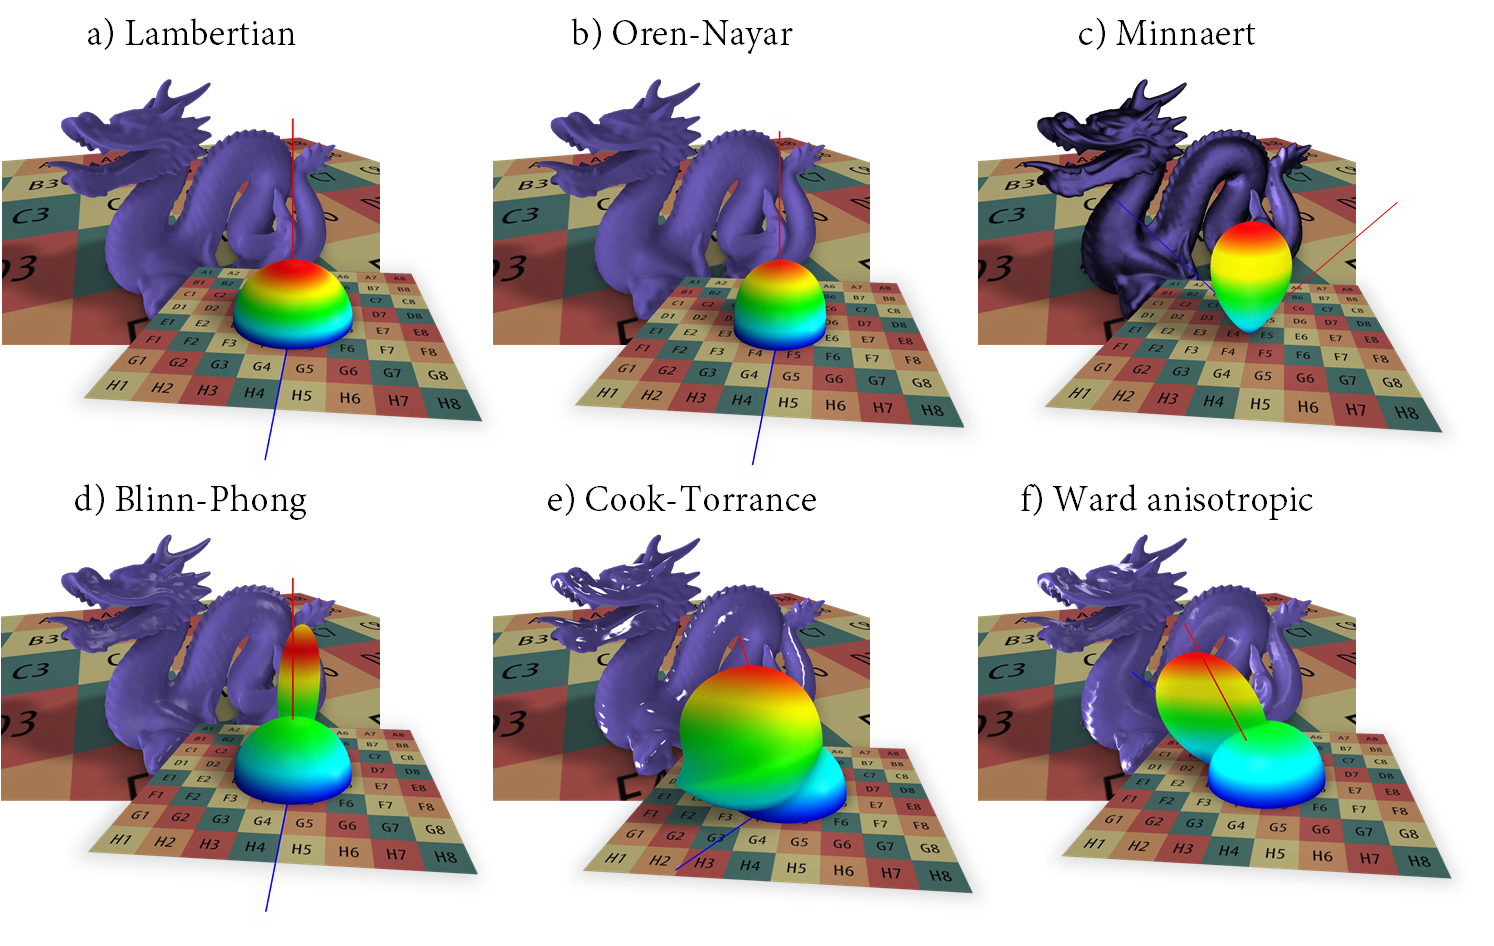
\includegraphics[width=\linewidth]{figs/lidar_intensity/analytical_brdfs.png}
    \caption{Some BRDFs depicted through their 3D plot and the rendering of a 3D model. $f_{r}(\vec{w})$ is represented by the distance from each vertex of the distorted semi-sphere to the origin, [0, 0, 0]. From left to right: a) Lambertian, b) Oren-Nayar with $\alpha_{m}$ = 0.5, c) Minnaert with a darkening factor ($k$) of 1.47, where as $\rho_{d}$ is increased by a factor of A = 2.6, d) Blinn-Phong with $\alpha$ = 11, e) Cook-Torrance with $\alpha$ = 0.685 and $F_{0}$ = 0.40, and f) Ward anisotropic with $\alpha_{x}$ = 0.15 and $\alpha_{y}$ = 0.75. $\rho_{d}$ = 1 for all the illustrated plots.  }
	\label{fig:lidar_analytical_brdfs}
\end{figure}

\section{Database BRDFs}

\begin{figure}
    \centering
    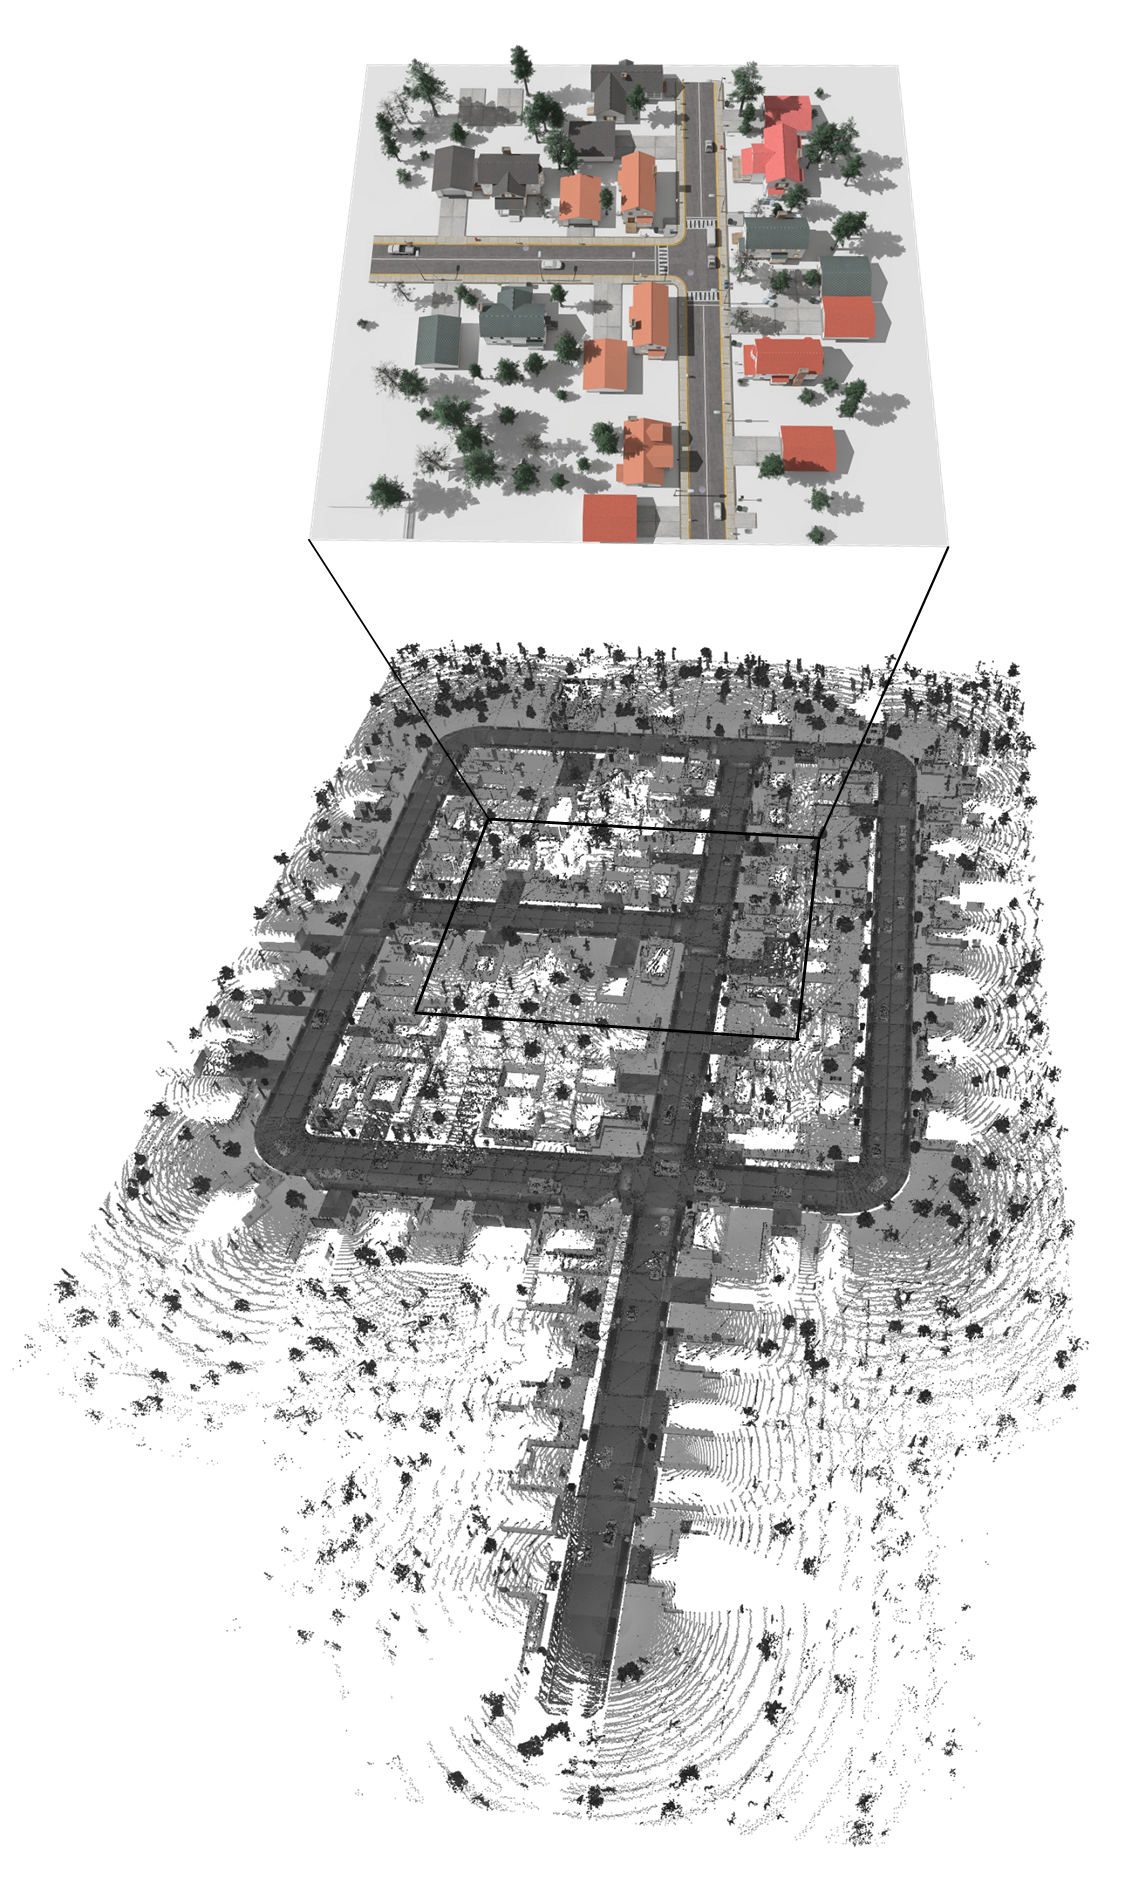
\includegraphics[width=\linewidth]{figs/lidar_intensity/material_database_intensity_results.png}
    \caption{Some BRDFs depicted.  }
	\label{fig:lidar_material_database_intensity_result}
\end{figure}

\section{Results and discussion}

The proposed simulation is evaluated using both high-performance and real LiDAR specifications. To this end, static and procedural scenes of high complexity (from 5M triangles to 11M) were used. The generated point clouds have been analyzed to provide better insight into semantic segmentation and intensity variability as the BRDF's properties change. We have also conducted large simulations to evaluate the response time of the GPU-based approach. A multi-core simulation in the CPU has been used as the reference method to measure latency improvements since recent work has not been published along with ready-to-run examples. Throughout this section, the LiDAR has either been configured as single/multiple return TLS, or multiple return ALS (up to five rebounds). Furthermore, they were set according to the specifications of notable commercial sensors, such as the Velodyne HDL-64E (TLS) or DJI Zenmuse L1 (ALS). However, the resolution and vehicle speed (e.g., a UAV for ALS) were modified to meet the requirements of high-performance tests. LiDAR's pulses were discretized using ten rays in all cases.

\subsection{Intensity measurement}

The emulation of different surfaces being reached by LiDAR beams is a key factor in this work. In the conducted tests, surfaces were linked to materials, whereas these materials were correlated with BRDF's profiles from \cite{dupuy_adaptive_2018} ($r$), refractive profiles ($\mu$) from \cite{mikhail_n_polyanskiy_refractive_nodate} and a roughness value ($\alpha$). Remark that the finally computed values also vary according to the model's materials. First, surfaces were linked to BRDFs that better represent their real behaviour, ranging from acrylic to metallic and anisotropic profiles. Then, the sensor wavelength is changed from 903\si{\nano\meter} to 532\si{\nano\meter}, thus obtaining lower intensity. Finally, all the surfaces were modelled with a BRDF similar to Lambertian, such as the one simulating maple leaf. The observed intensity is depicted in Figure \ref{fig:database_intensity_results} through histograms for different types of LiDAR surveys and materials, using as input a procedurally populated scene.

\begin{figure*}[ht]
	\centering
	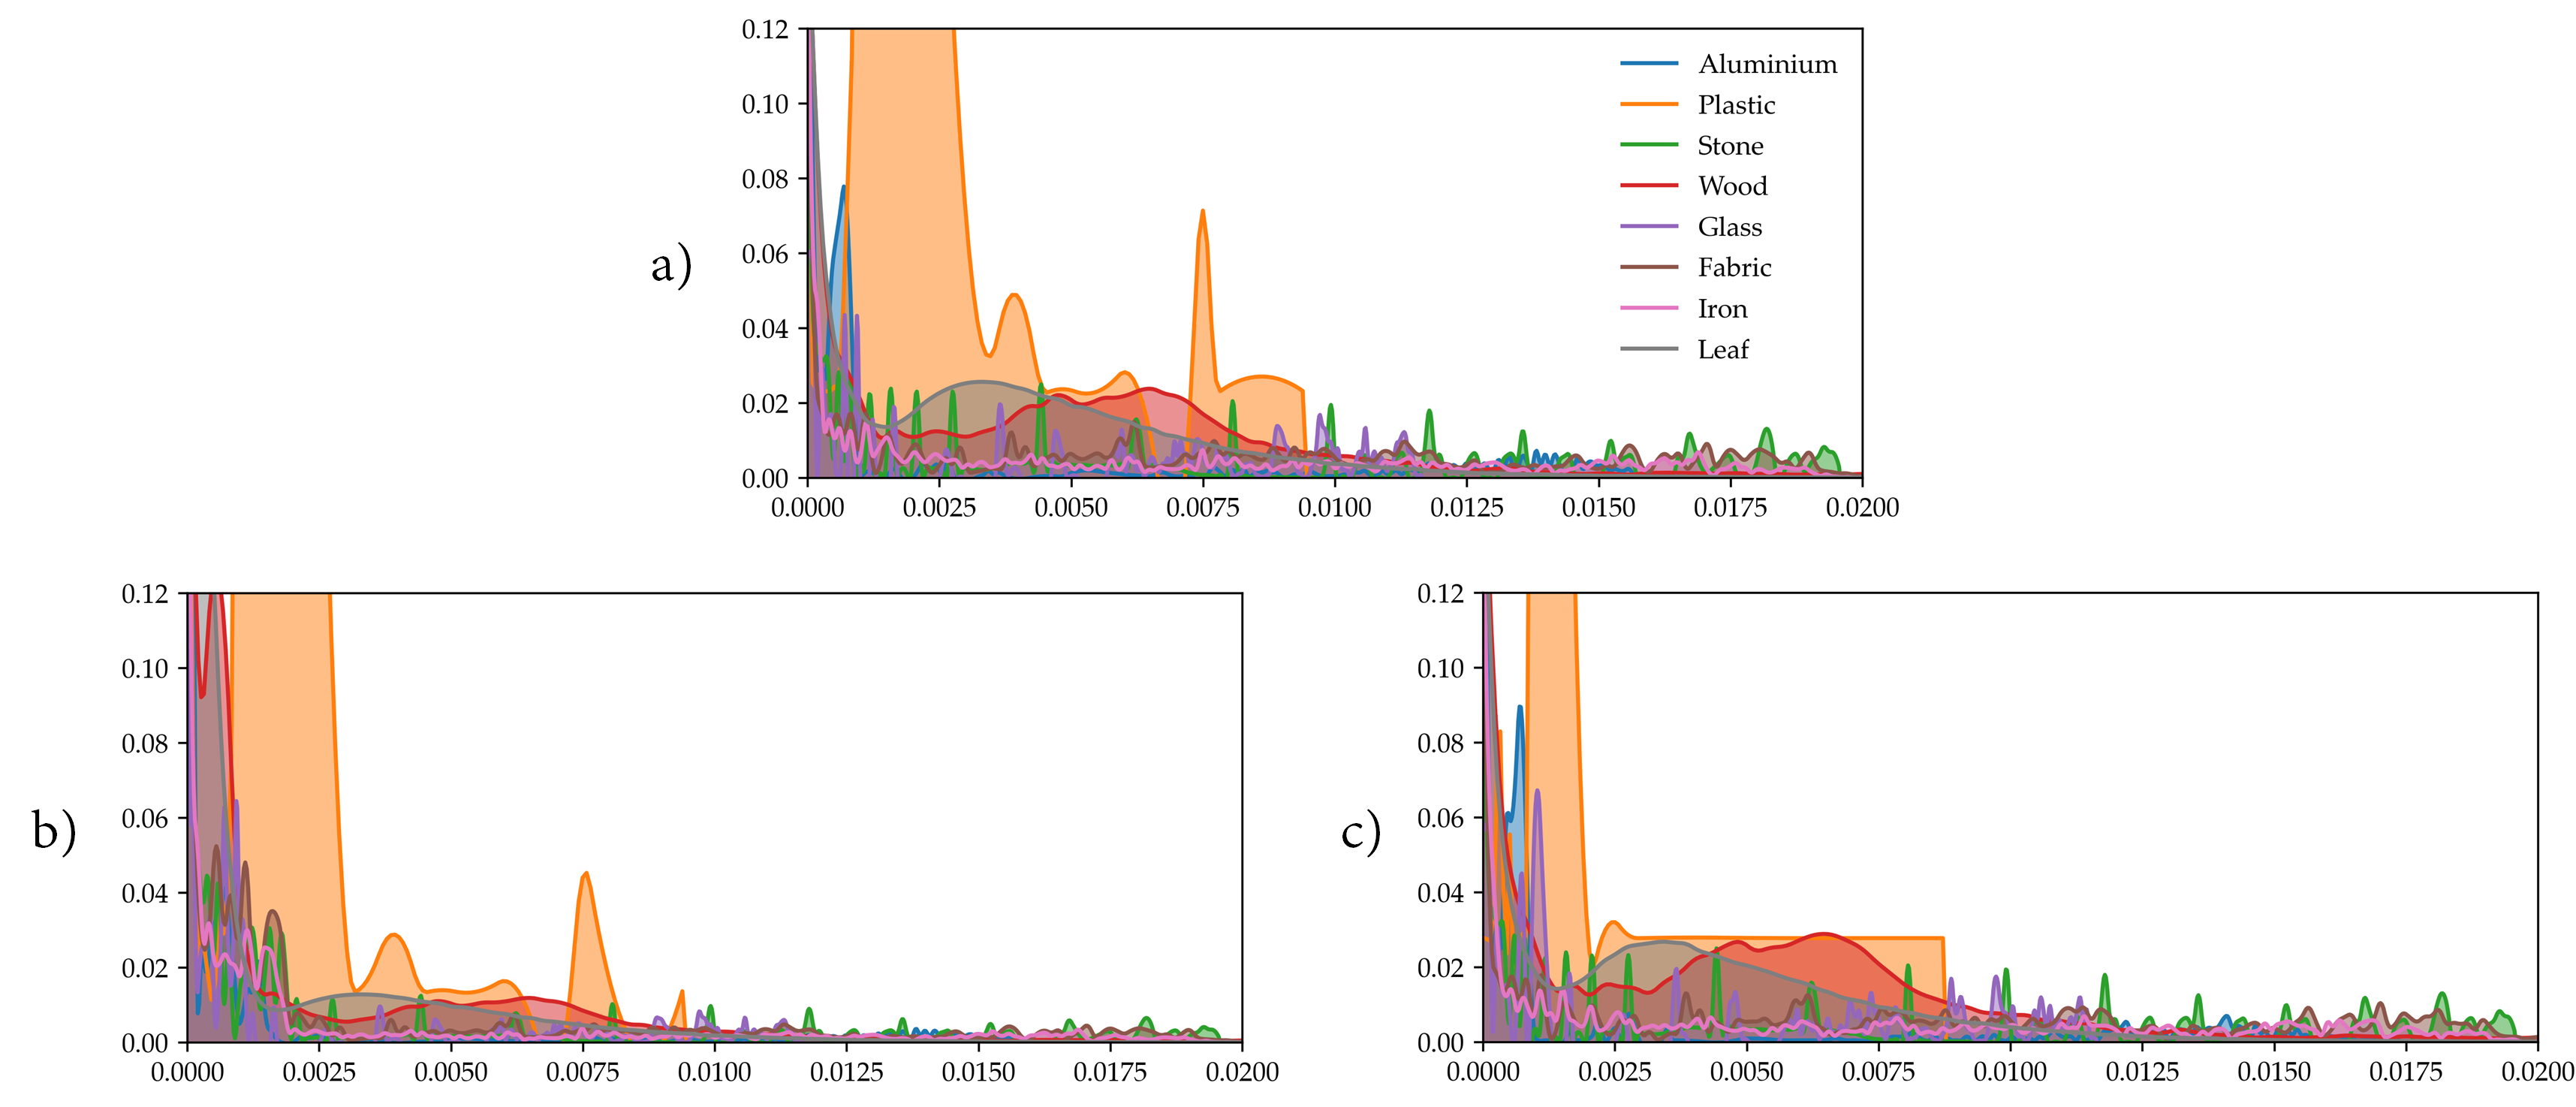
\includegraphics[width=\linewidth]{figs/lidar_intensity/database_intensity_chart.png}
	\caption{From top to bottom: intensity from the simulation of an HDL-64E LiDAR working at 903\si{\nano\meter} and surfaces with realistic materials, idem with LiDAR working at 532\si{\nano\meter} and the first simulation with all the surfaces represented as Lambertian.}
	\label{fig:database_intensity_results}
\end{figure*}

The distribution of intensity over $[0, 1]$ varies depending both on the surface BRDF and the normal vector. Hence, histograms from aerial surveys show a Gaussian form, since a wider variety of normal vectors are sampled. On the other hand, terrestrial results are more unbalanced as a result of a narrow field of view. Using only Lambertian surfaces, the intensity values are more uniformly distributed, although histograms vary as a consequence of distance and observed normals. However, surveys with either a high wavelength or diffuse-like materials present a brighter signature.

\subsection{Intensity measurement}

Another key factor in the proposed framework is the emulation of surface behaviour for striking beams. The surfaces are first linked to a material similar to their behaviour in nature, according to our material database. Then, all surfaces are represented as Lambertian. For the first assignment, materials and BRDFs are linked as follows: \verb|Aluminium| $\gets$ \verb|Cook-Torrance|, \verb|Glass| $\gets$ \verb|Blinn-Phong|, \verb|Fabric| $\gets$ \verb|Minnaert|, \verb|Iron| $\gets$ \verb|Cook-Torrance|, \verb|Leaf| $\gets$ \verb|Oren-Nayar|, \verb|Plastic| $\gets$ \verb|Cook-Torrance|, \verb|Stone| $\gets$ \verb|Minnaert|, \verb|Wood| $\gets$ \verb|Ward Anisotropic|, whereas Lambert model is assigned to the rest. Intensity is depicted in Figure \ref{fig:analytical_brdf_results} through histograms for different types of LiDAR surveys and materials, using as input a procedurally populated scene.

\begin{figure*}[ht]
	\centering
	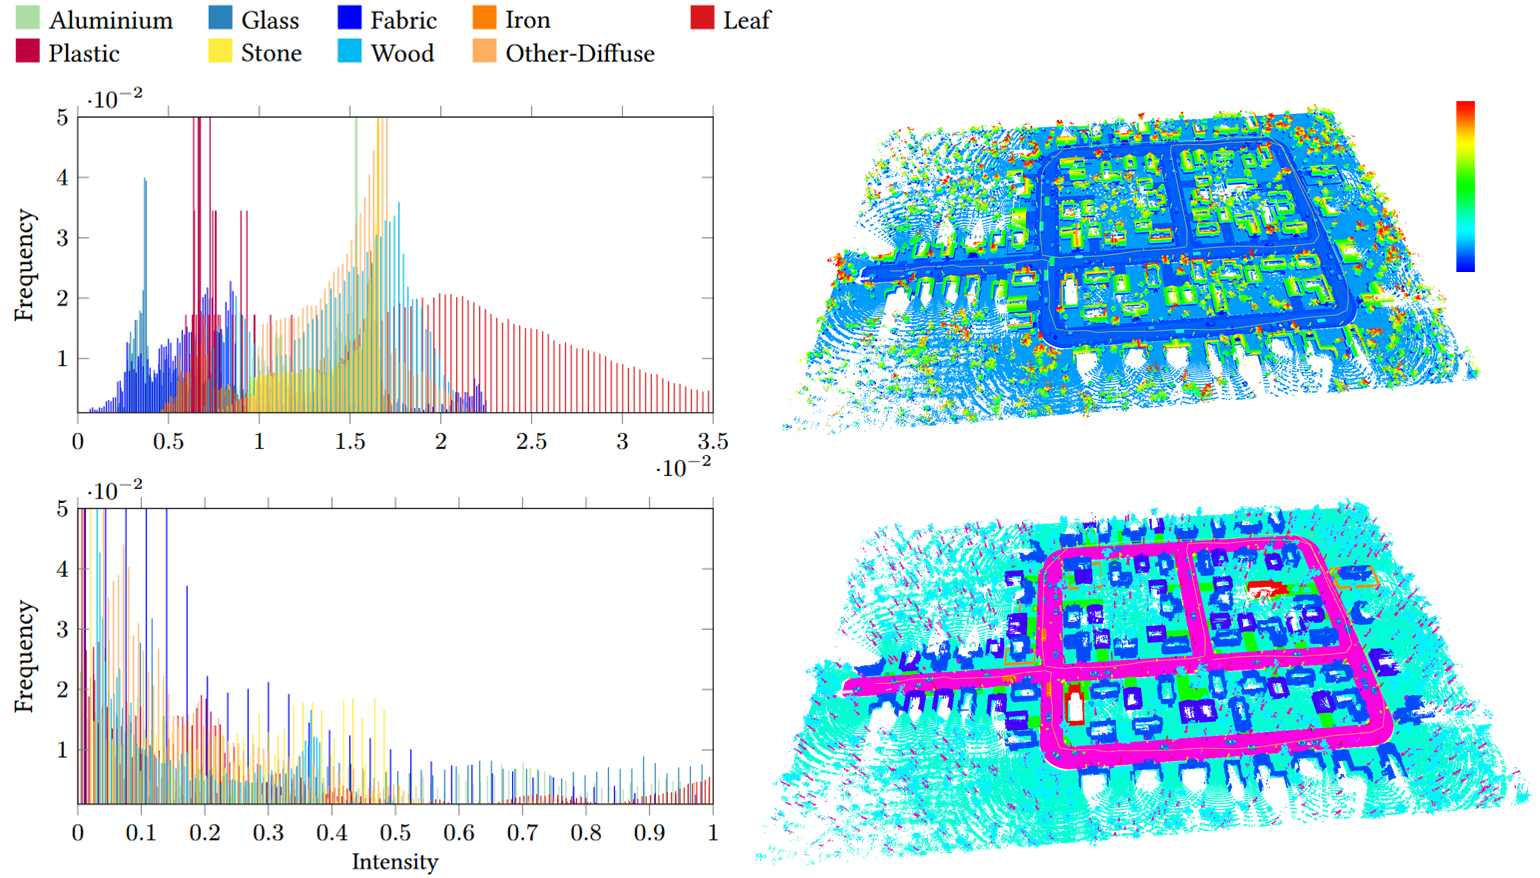
\includegraphics[width=\linewidth]{figs/lidar_intensity/analytical_brdf_intensity_chart.png}
	\caption{Intensity comparison of two procedural environments with different BRDF distributions for an aerial simulation. a) Objects receive the most accurate BRDF in comparison with their real behaviour, whereas b) uses a Lambertian model for every surface. Right images shows the same point cloud rendered according to their relative height and semantic labels, respectively.}
	\label{fig:analytical_brdf_results}
\end{figure*}

The distribution of intensity over $[0, 1]$ varies depending both on the surface BRDF and the normal vector. Hence, histograms from aerial surveys show a Gaussian form, since a wider variety of normal vectors are sampled. On the other hand, terrestrial results are more unbalanced as a result of a narrow field of view. Using only Lambertian surfaces, the intensity values are more uniformly distributed, although histograms vary as a consequence of distance and observed normals. However, similarly to Figure \ref{fig:analytical_brdf_results}, materials following diffuse BRDFs, e.g. Minnaert, present a brighter signature when represented as Lambertian.

\section{Conclusions and future work}

In this paper, we proposed a GPU-based LiDAR simulator for generating semantic BRDF-aware point clouds. Furthermore, it includes multiple returns and well-known LiDAR errors. To this end, LiDAR's pulses were discretized as several rays that strike into the scene surfaces, instead of solving the simulation in the image space. This procedure was implemented in GLSL and compared with its analogous multi-core CPU approach by conducting much more dense scans than actual LiDAR sensors. These tests showed that the GPU approach improves the sequential procedure with speedups above 90\%. Thus, the described algorithm is suitable both for real-time simulations and the generation of large LiDAR semantic point clouds with low latency. Accordingly, LiDAR sessions can be solved iteratively or in a single batch. Also, the sensor parameterization allows simulating a wide range of LiDAR sensors and platforms, including ALS.

In future work, we would like to enhance the proposed methodology using distributed systems. Furthermore, we aim to extend this framework to full-waveform and single-photon LiDAR \cite{tachella_real-time_2019} and other yet nonincluded systems. Regarding Deep Learning applications, a deeper study ought to be conducted to show the benefits of using virtual LiDARs over procedural environments to generate semantic LiDAR datasets. Finally, it provides the possibility of generating datasets for every kind of scenario, from forestry to urban environments for autonomous navigation.